%-*- coding: UTF-8 -*-
% notes.tex
%
\documentclass[UTF8]{article}
\usepackage{geometry}
\geometry{a4paper, centering, scale=0.8}
\usepackage{minted}
\usepackage{hyperref}
\usepackage{indentfirst}    % to indent the first paragraph of a section
\usepackage{graphicx}       % to insert figures
\usepackage{amsmath}        % to type some math equations
\usepackage{amssymb}        % to use some special math font
\usepackage{IEEEtrantools}  % to use IEEEeqnarray
\usepackage{algorithm2e}    % to use algorithm environment
\usepackage{mathtools}      % to use \lfloor etc.
\usepackage{multicol}       % to display some content in multi-columns
\setlength{\columnseprule}{0.4pt}   % set the rule's width of multicols
\setlength{\columnsep}{5em}         % set the sep of multicols

% Math notation
% refered to https://github.com/exacity/deeplearningbook-chinese/blob/master/math_symbol.tex
\newcommand{\Scalar}[1]{\mathit{#1}}                % Scalar, the default math font
\newcommand{\Vector}[1]{\boldsymbol{\mathit{#1}}}   % Vector
\newcommand{\Matrix}[1]{\boldsymbol{\mathit{#1}}}   % Matrix
\newcommand{\Tensor}[1]{\textsf{\textbf{#1}}}       % Tensor
\newcommand{\Set}[1]{\mathbb{#1}}                   % Set
\newcommand{\Cal}[1]{\mathcal{#1}}                  % Math Cal

% Draw the lines in a matrix, which is composed by a series of vectors
\newcommand{\vRule}{\rule{0.3pt}{10mm}}             % vertical rule
\newcommand{\hRule}{\,\rule[1mm]{10mm}{0.3pt}\,}    % horizontal rule

% Ceil and floor
\DeclarePairedDelimiter\ceil{\lceil}{\rceil}
\DeclarePairedDelimiter\floor{\lfloor}{\rfloor}

\title{Deep Learning Specialization \\
        Convolutional Neural Networks}
\author{Du Ang \\ \texttt{du2ang233@gmail.com} }
\date{\today}

\begin{document}
\maketitle

\tableofcontents
\newpage

\section{Foundations of Convolutional Neural Networks}
\subsection{Convolutional Neural Networks}
\subsubsection{Computer Vision}
\paragraph{Computer Vision problems}
\begin{itemize}
    \item Image Classfiication
    \item Object Detection
    \item Neural Style Transfer
\end{itemize}

One of the challenges of Computer Vision problems is that the input can be really big. We want to
use large images to train our model, and if we use a fully-connected network, the huge input
features and so many parameters are not feasible to train.

\subsubsection{Edge Detection Example}
\paragraph{Vertical edge detection}
The convolution operation in programming languages:
\begin{itemize}
    \item Python: \mintinline{python}{conv_forward}
    \item TensorFlow: \mintinline{python}{tf.nn.conv2d}
\end{itemize}

\begin{figure}[htb]
    \centering
    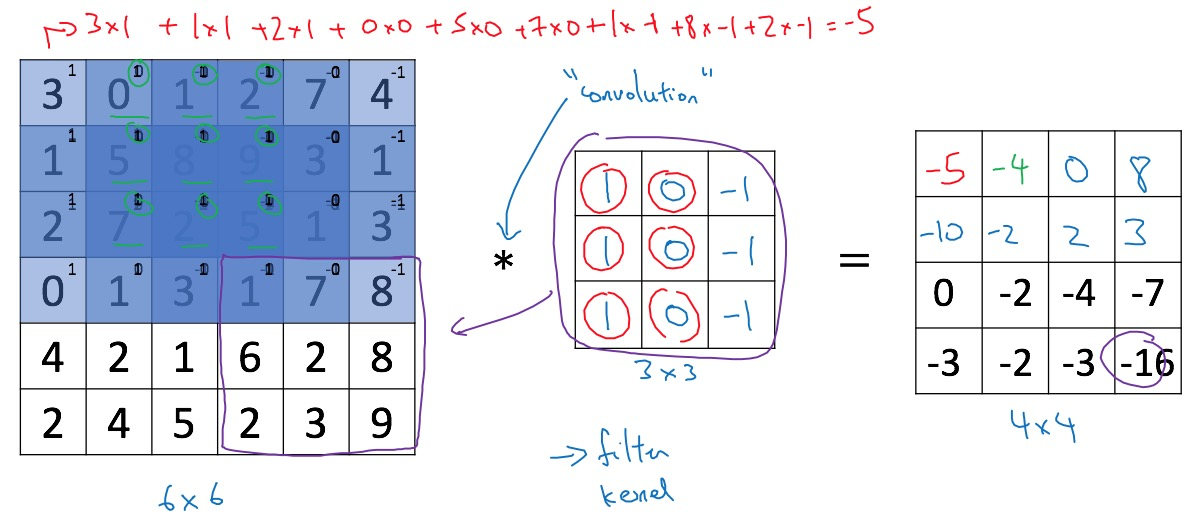
\includegraphics[width=40em]{figures/convolution-operation}
    \caption{The convolution operation for vertical edge detection}
    \label{fig:convolution-operation}
\end{figure}

\begin{figure}[htb]
    \centering
    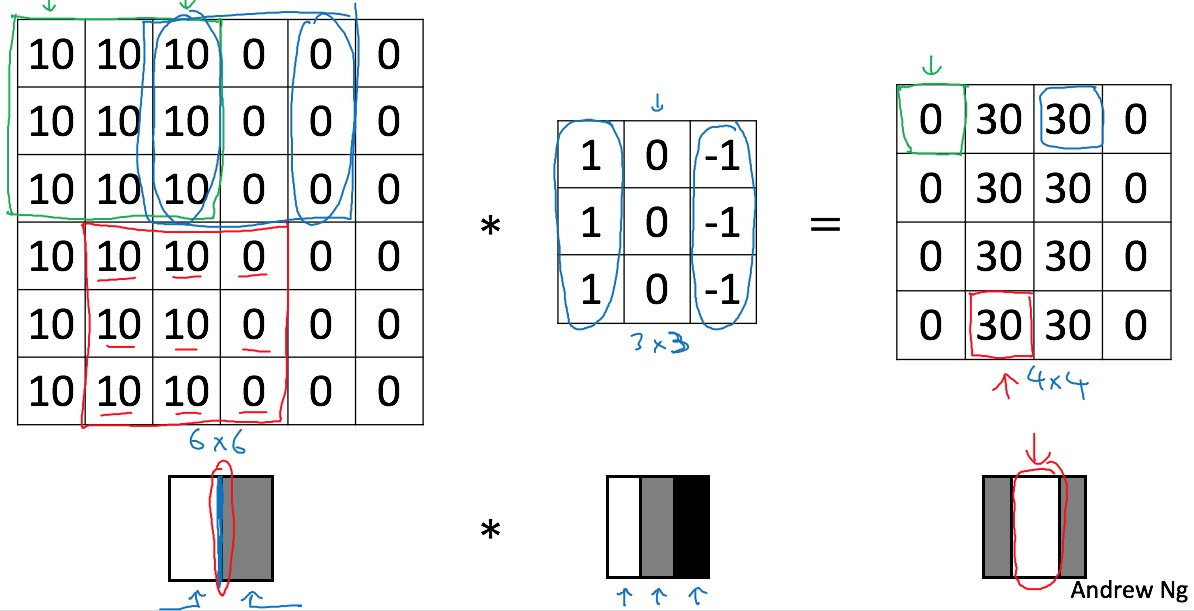
\includegraphics[width=40em]{figures/vertical-edge-detection-example}
    \caption{Vertical edge detection example for a simplified image}
    \label{fig:vertical-edge-detection-example}
\end{figure}

\subsubsection{More Edge Detection}
\begin{figure}[htb]
    \centering
    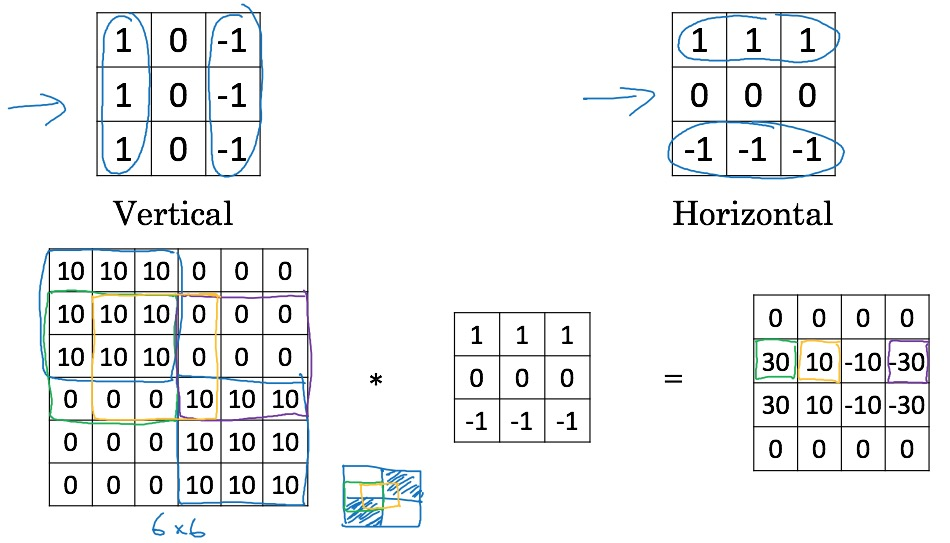
\includegraphics[width=40em]{figures/vertical-and-horizontal-edge-detection-example}
    \caption{Vertical and horizontal edge detection example}
    \label{fig:vertical-and-horizontal-edge-detection-example}
\end{figure}

\paragraph{Learning to detect edges}
Like Figure~\ref{fig:learning-to-detect-edges} shows, the idea that you can treat the nine numbers
in the filter as parameters, has been one of the most powerful ideas in computer vision.

\begin{figure}[htb]
    \centering
    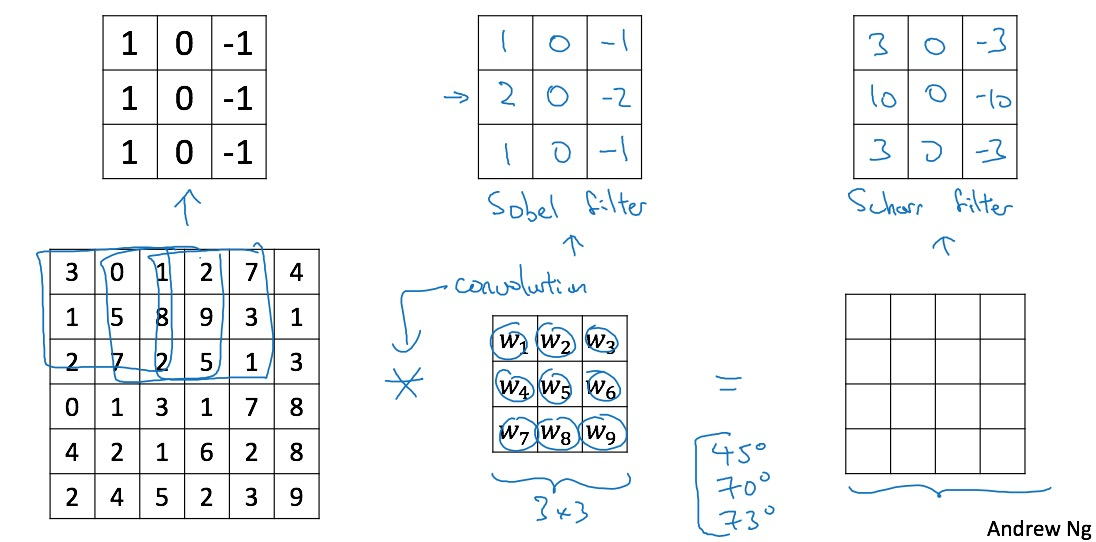
\includegraphics[width=40em]{figures/learning-to-detect-edges}
    \caption{Edge detection example with parameters to learn}
    \label{fig:learning-to-detect-edges}
\end{figure}

\subsubsection{Padding}
For a $n \times n$ image, use a $f \times f$ filter to do convolution, we will get a $(n-f+1) \times
(n-f+1)$ output.

The problems of no padding:
\begin{itemize}
    \item shrinking output
    \item throwing away information from edge
\end{itemize}

\paragraph{Valid and Same convolutions}
\begin{itemize}
    \item ``Valid'': $n \times n \* f \times f \rightarrow (n-f+1) \times (n-f+1)$
    \item ``Same'': Pad so that output size is the same as the input size.
    If we add padding $p$, the output will be $(n+2p-f+1) \times (n+2p-f+1)$, $\displaystyle
    p = \frac{f-1}{2}$. In convention, $f$ is usually odd.
\end{itemize}

\subsubsection{Strided Convolutions}
Strided convolutions is another piece of the basic builiding block of convolutions as used in
convolutional neural networks.

\begin{figure}[htb]
    \centering
    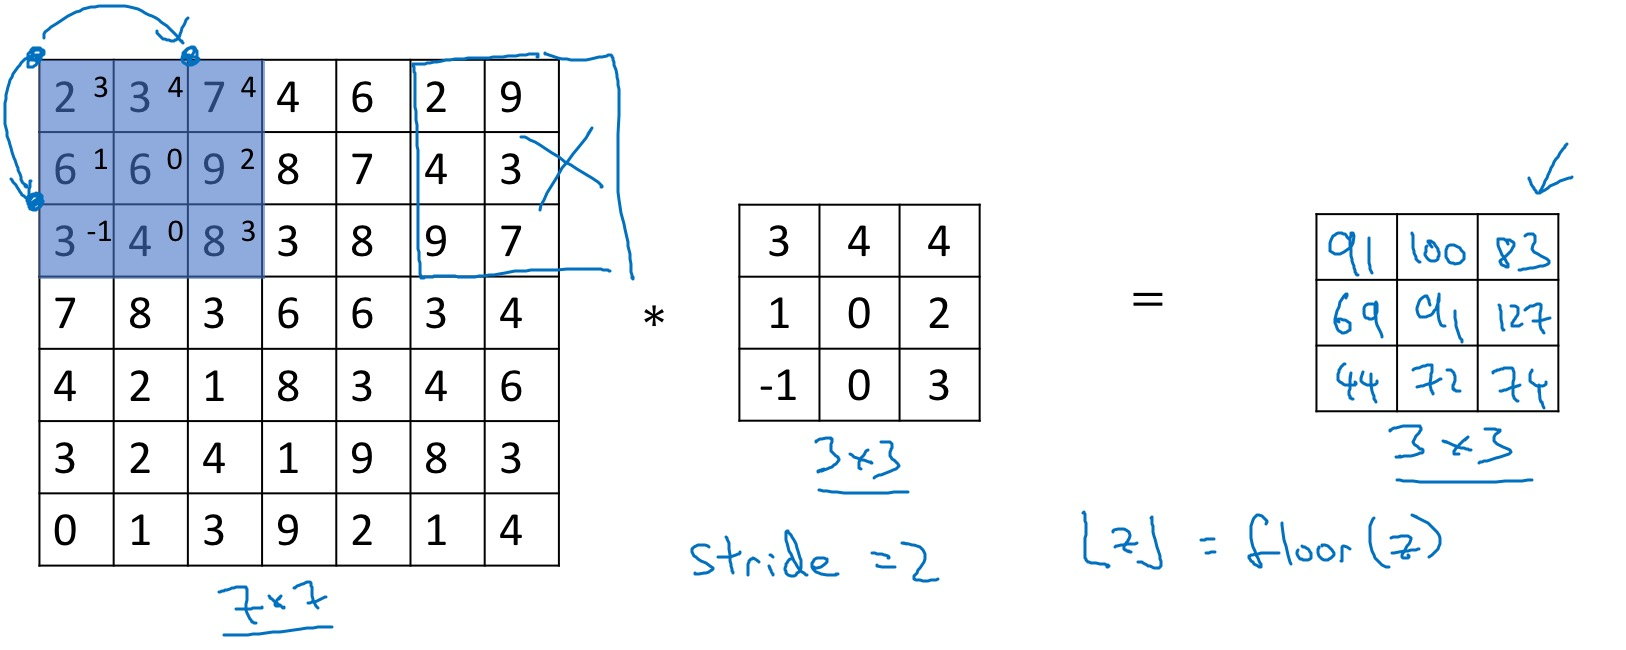
\includegraphics[width=40em]{figures/strided-convolution}
    \caption{Strided convolution example with stride 2}
    \label{fig:strided-convolution}
\end{figure}

$$ n \times n \text{ image (padding } p \text{)} \quad * \quad f \times f \text{ filter (stride }
s \text{)}  \quad \rightarrow \quad \floor*{\frac{n+2p-f}{s}+1} \times \floor*{\frac{n+2p-f}{s}+1}$$

\paragraph{Technical note on cross-correlation vs. convolution}
Convolution in math textbook and sigal processing has an extra mirroring operation, but in Deep
Learning, we've skipped it by convention. Technically, what we're actually doing, is sometimes
called cross-correlation instead of convolution.

The real convolution has the property called associativity in mathematics, which means $(A * B) * C
= A * (B * C)$. This is nice for some signal processing applications, but for deep neural networks,
it really doesn't matter.

\subsubsection{Convolutions Over Volume}
Figure~\ref{fig:convolutions-on-rgb-image} shows the example of convolutions over volume.

\begin{figure}[htb]
    \centering
    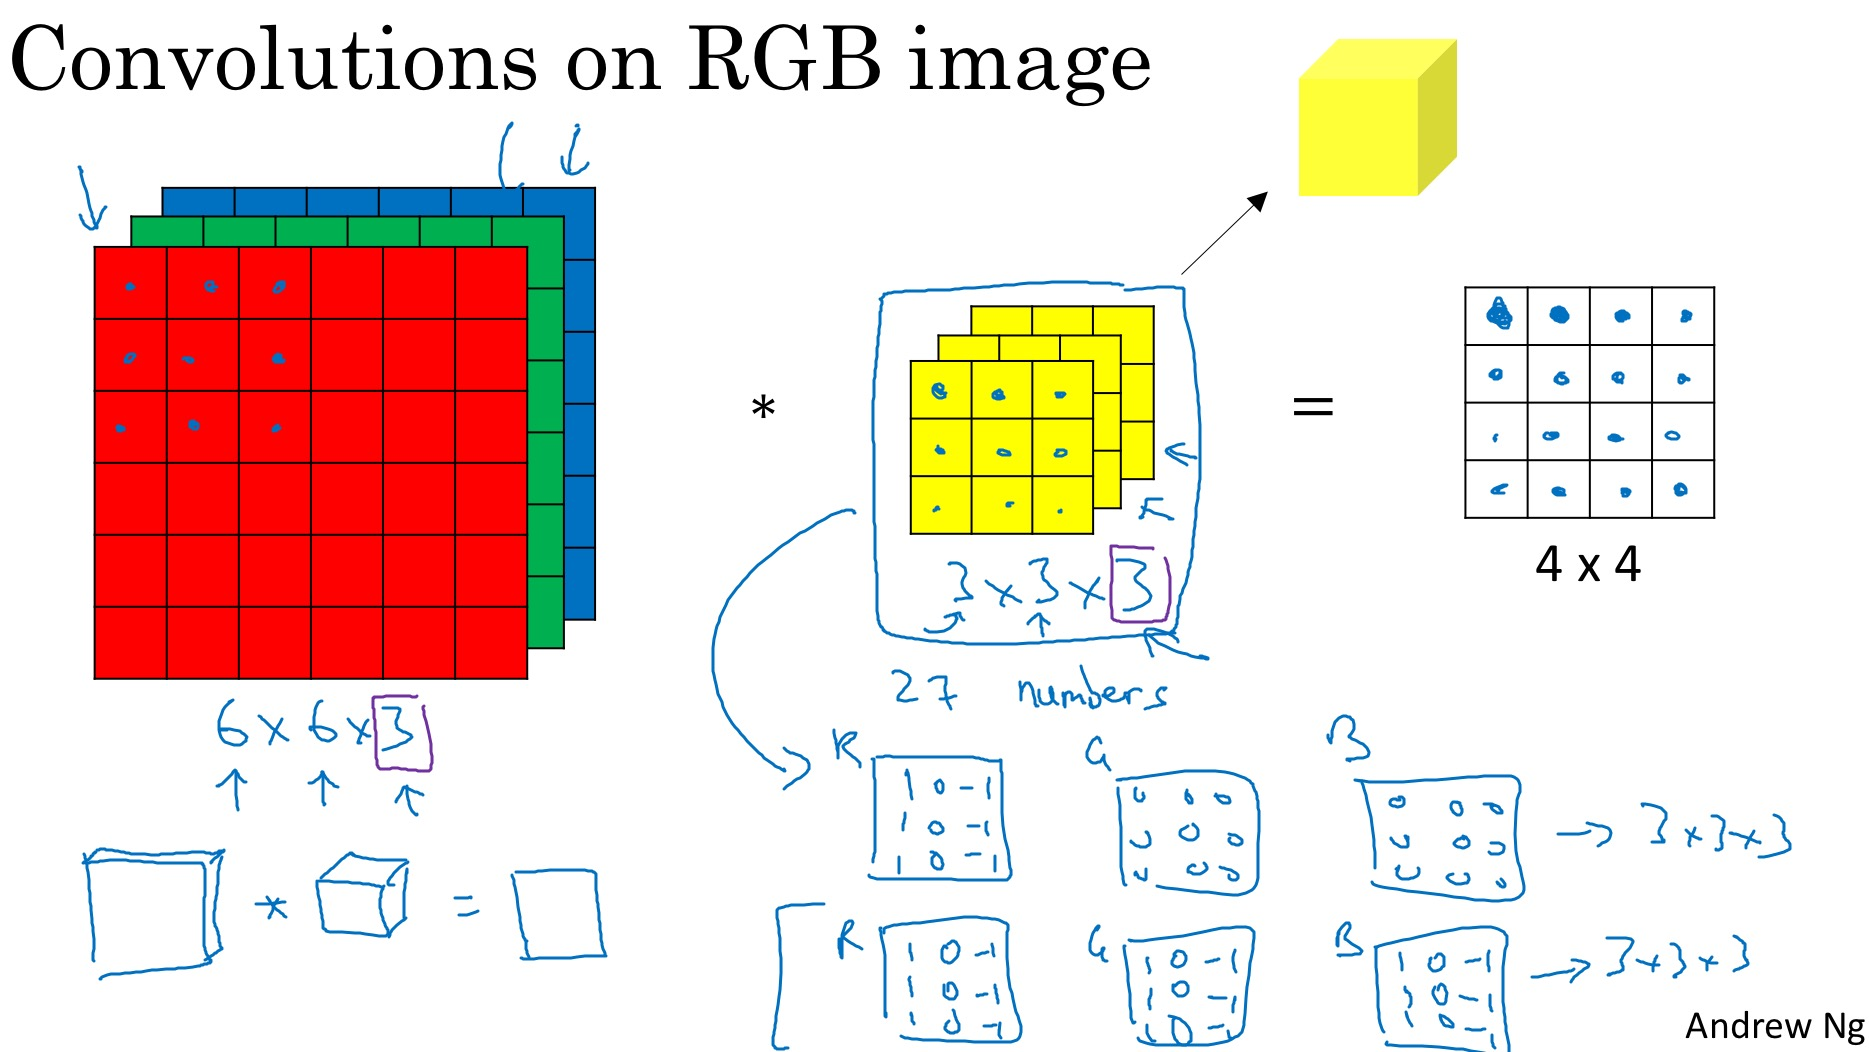
\includegraphics[width=40em]{figures/convolutions-on-rgb-image}
    \caption{Convolutions on RGB image}
    \label{fig:convolutions-on-rgb-image}
\end{figure}

If we want to detect different features at the same time, we can use multiple filters. The output
will then have a number of channels equal to the features you are detecting.

Sometimes, the term ``channel'' is also called ``depth''.

\paragraph{Summary}
$$ n \times n \times n_C \quad * \quad f \times f \times n_C \quad \rightarrow \quad
(n-f+1) \times (n-f+1) \times n_C' \qquad (stride = 1, \text{no padding})$$

\subsubsection{One Layer of a Convolutional Network}
Figure~\ref{fig:example-of-a-conv-layer} shows an example of a layer of a convolutional network.

\begin{figure}[htb]
    \centering
    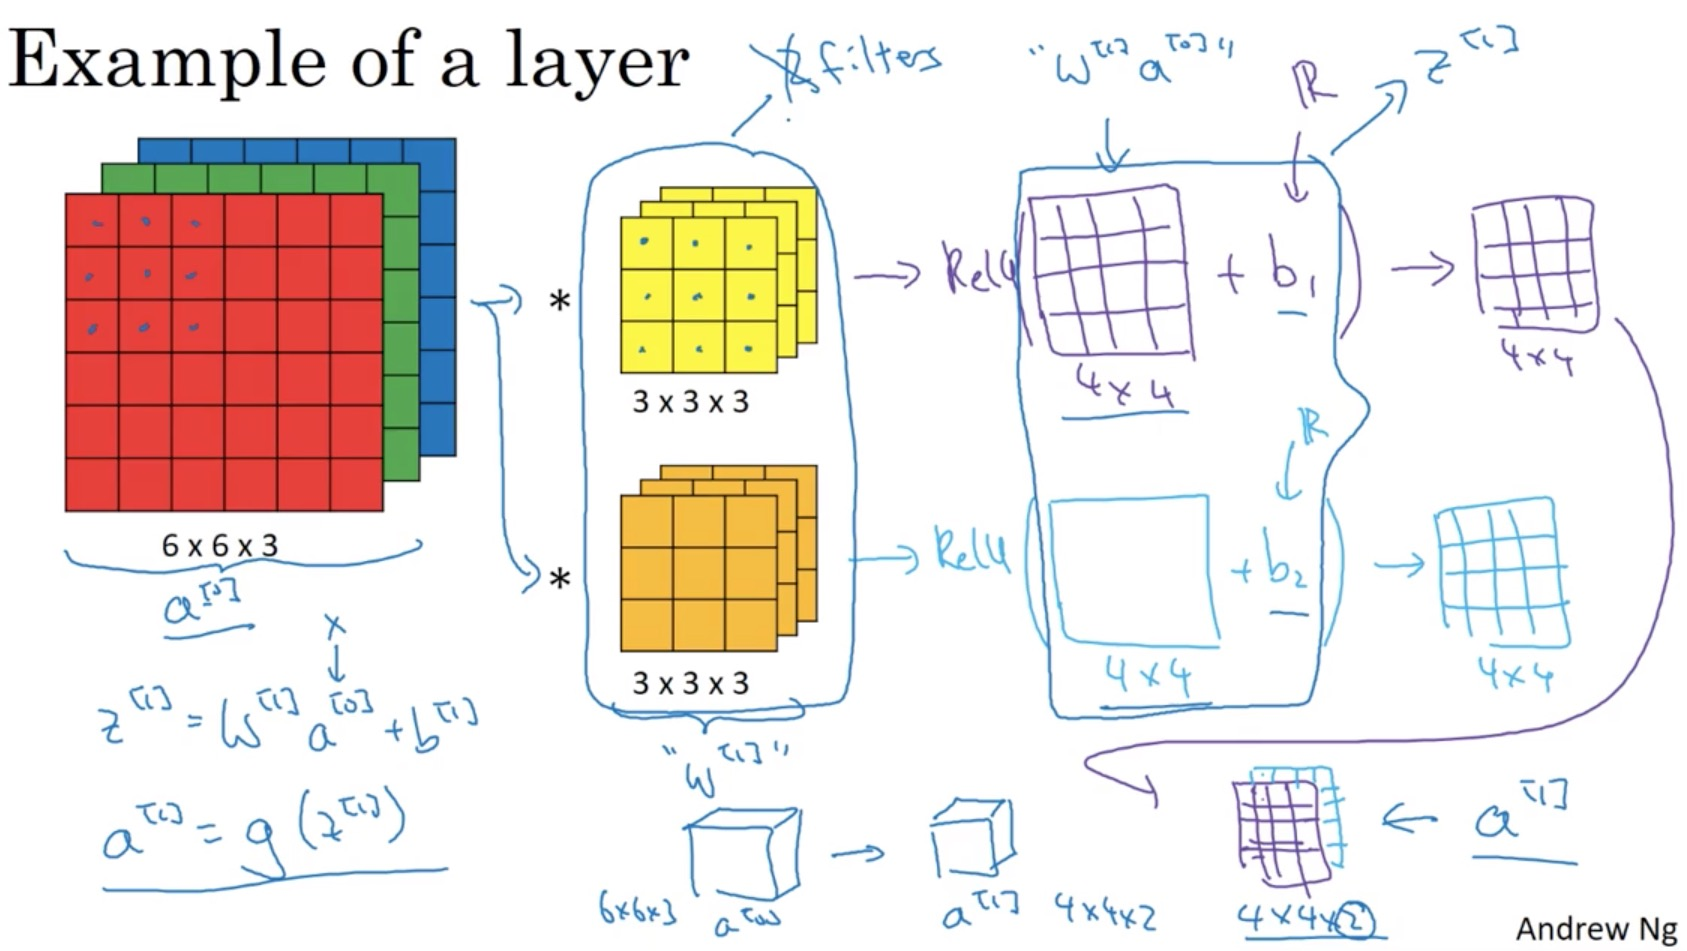
\includegraphics[width=40em]{figures/example-of-a-conv-layer}
    \caption{A example of a convolutional layer}
    \label{fig:example-of-a-conv-layer}
\end{figure}

\paragraph{Number of parameters in one layer}
If you have 10 filters that are $3 \times 3 \times$ in one layer of a neural network, how many
parameters does that layer have?
$$ (3 \times 3 \times 3 + 1) \times 10 = 280 $$

\paragraph{Summary of notation}
If layer $l$ is a convolution layer:
\begin{itemize}
    \item $f^{[l]} = \text{filter size}$
    \item $p^{[l]} = \text{padding}$
    \item $s^{[l]} = \text{stride}$
    \item $n_{\text{C}}^{[l]} = \text{number of filters}$
    \item Each filter is: $f^{[l]} \times f^{[l]} \times n_{\text{C}}^{[l]}$
    \item Activations: $\Vector{a}^{[l]} \rightarrow n_{\text{H}}^{[l]} \times n_{\text{W}}^{[l]} \times
    n_{\text{C}}^{[l]} \qquad \Matrix{A}^{[l]} \rightarrow m \times n_{\text{H}}^{[l]} \times
    n_{\text{W}}^{[l]} \times n_{\text{C}}^{[l]}$
    \item Weights: $f^{[l]} \times f^{[l]} \times n_{\text{C}}^{[l]} \times n_{\text{C}}^{[l-1]}$
    \item bias: $n_{\text{C}}^{[l]} \rightarrow (1, 1, 1, n_{\text{C}}^{[l]})$
    \item Input: $n_{\text{H}}^{[l-1]} \times n_{\text{W}}^{[l-1]} \times n_{\text{C}}^{[l-1]}$
    \item Output: $n_{\text{H}}^{[l]} \times n_{\text{W}}^{[l]} \times n_{\text{C}}^{[l]}$
    \item $\displaystyle n_{\text{H/W}}^{[l]} = \floor{\frac{n_{\text{H/W}}^{[l-1]} + 2p^{[l]}
    - f^{[l]}}{s^{[l]}} + 1}$
\end{itemize}

\subsubsection{Simple Convolutional Network Example}
A simple convolutional network example can be seen in Figure~\ref{fig:example-of-a-conv-layer}.

As you go deeper in the neural network, typically you start up with larger images, the height
and width will stay the same for a while, and gradually trend down as you go deeper in your
networks, whereas the number of channels will generally increase.

\begin{figure}[htb]
    \centering
    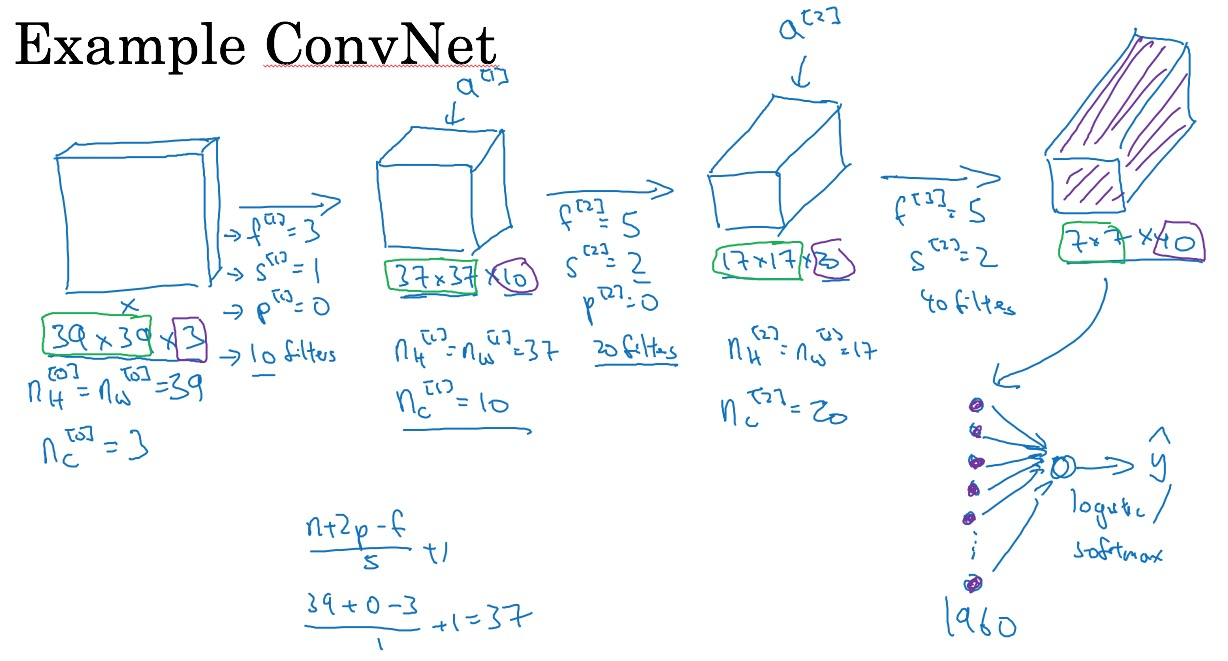
\includegraphics[width=40em]{figures/example-of-a-conv-net}
    \caption{A example of a convolutional network}
    \label{fig:example-of-a-conv-layer}
\end{figure}

Types of layers in a convolutional network:
\begin{itemize}
    \item Convolution (CONV)
    \item Pooling (POOL)
    \item Fully connected (FC)
\end{itemize}

\subsubsection{Pooling Layers}
Figure~\ref{fig:max-pooling} shows what max pooling is. As you can see, each coloured moving window
captures the maximum value within the widow is the output.

\begin{figure}[htb]
    \centering
    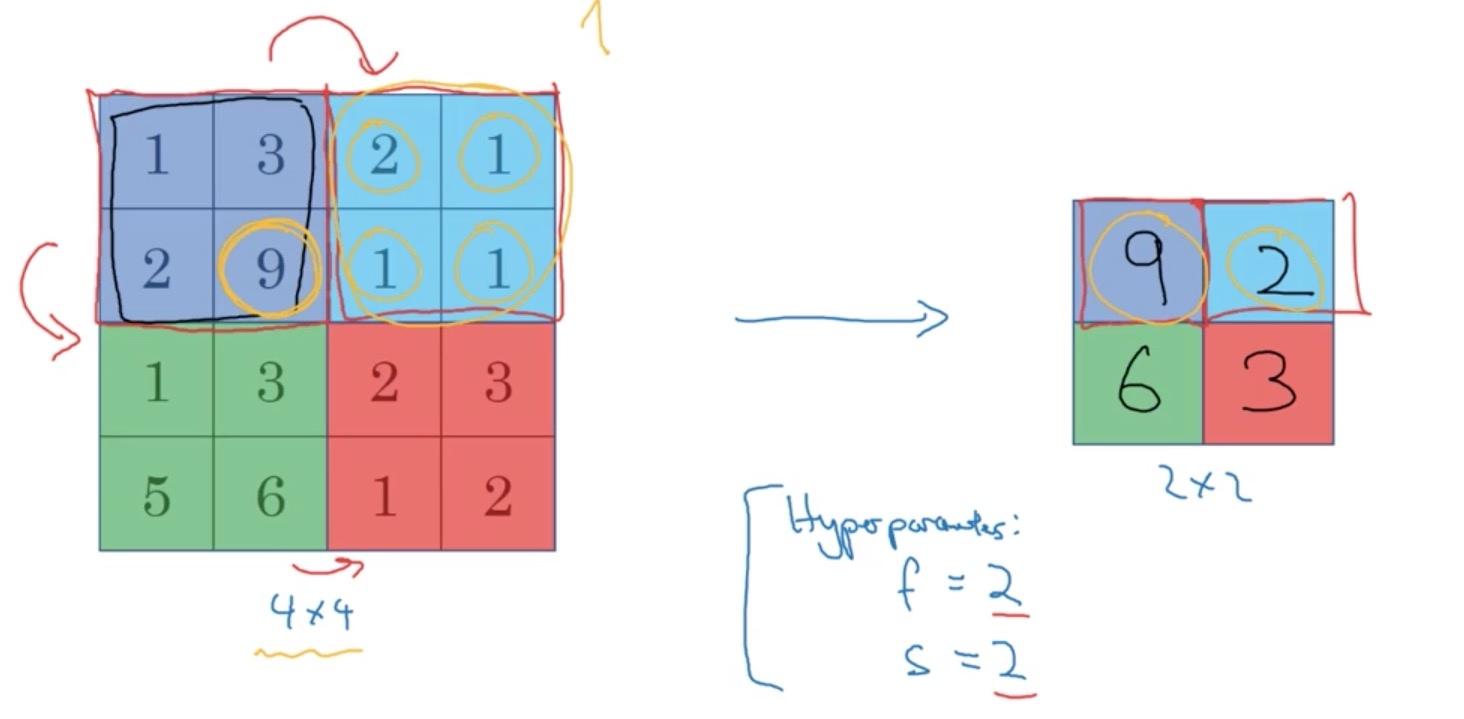
\includegraphics[width=40em]{figures/max-pooling}
    \caption{Max pooling}
    \label{fig:max-pooling}
\end{figure}

Figure~\ref{fig:average-pooling} shows a average pooling example. Instead of taking the maxes
within each filter, you take the average.

\begin{figure}[htb]
    \centering
    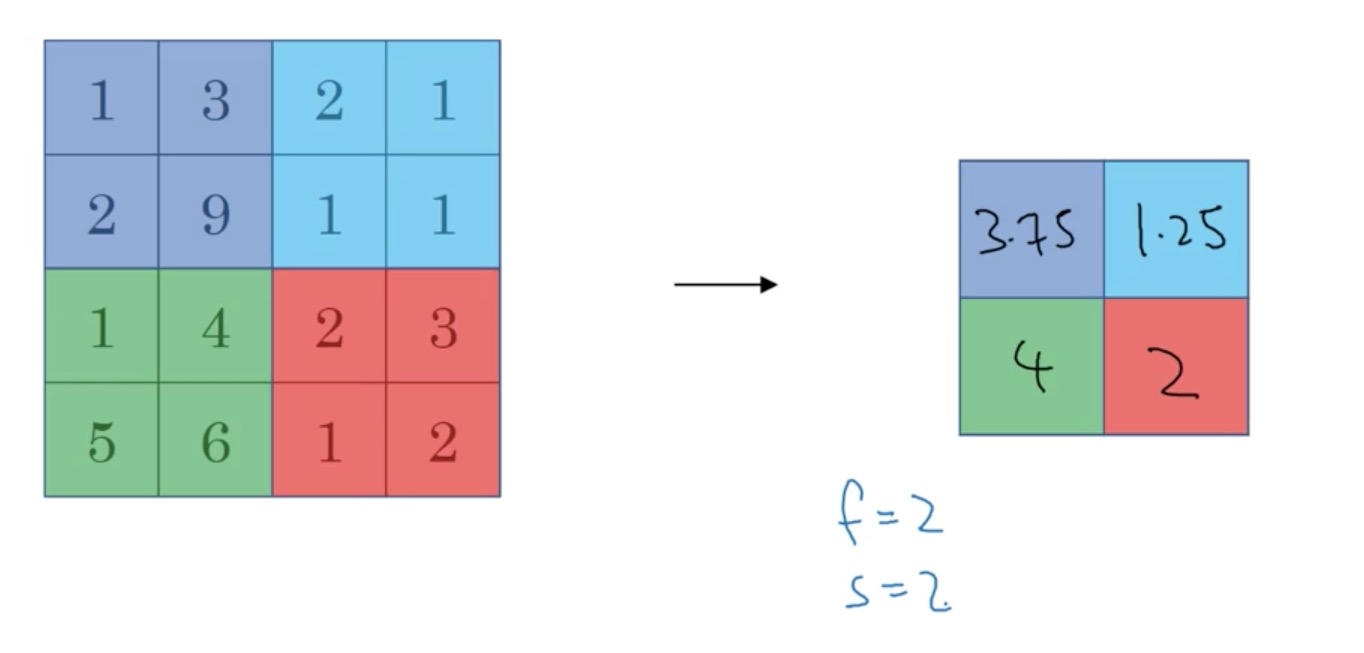
\includegraphics[width=40em]{figures/average-pooling}
    \caption{Average pooling}
    \label{fig:average-pooling}
\end{figure}

These days max pooling is used much more often than average pooling. With one exception, which is
sometimes, very deep in a neural network, you might use average pooling to collapse your
implementation from, say, $7 \times 7 \times 1000$, and average over all to get $1 \times 1 \times
1000$.

Hyperparameters (max or average pooling):
\begin{itemize}
    \item $f$: \text{filter size}
    \item $s$: \text{stride}
    \item ($p$: \text{padding}, little used)
\end{itemize}

Input: $ n_{\text{H}} \times n_{\text{W}} \times n_{\text{C}} $

Output: $\displaystyle \floor*{\frac{n_{\text{H}}-f}{s}+1} \times
\floor*{\frac{n_{\text{W}}-f}{s}+1} \times n_{\text{C}} $

Pooling layers have no parameters to learn.

\subsubsection{CNN Example}
Figure~\ref{fig:cnn-example} shows a CNN example inpired by LeNet-5.

In the literature of a Conv net, there are two conventions which are slightly in consistence about
what you call a layer. One convention is call CONV+POOL a layer. Another convention would be to
count the CONV layer as a layer, and the POOL layer as a layer. When people report a number of
layers in a neural network, usually people report just the number of layers that have weights
(parameters). In this class, we will use the first convention.

\begin{figure}[htb]
    \centering
    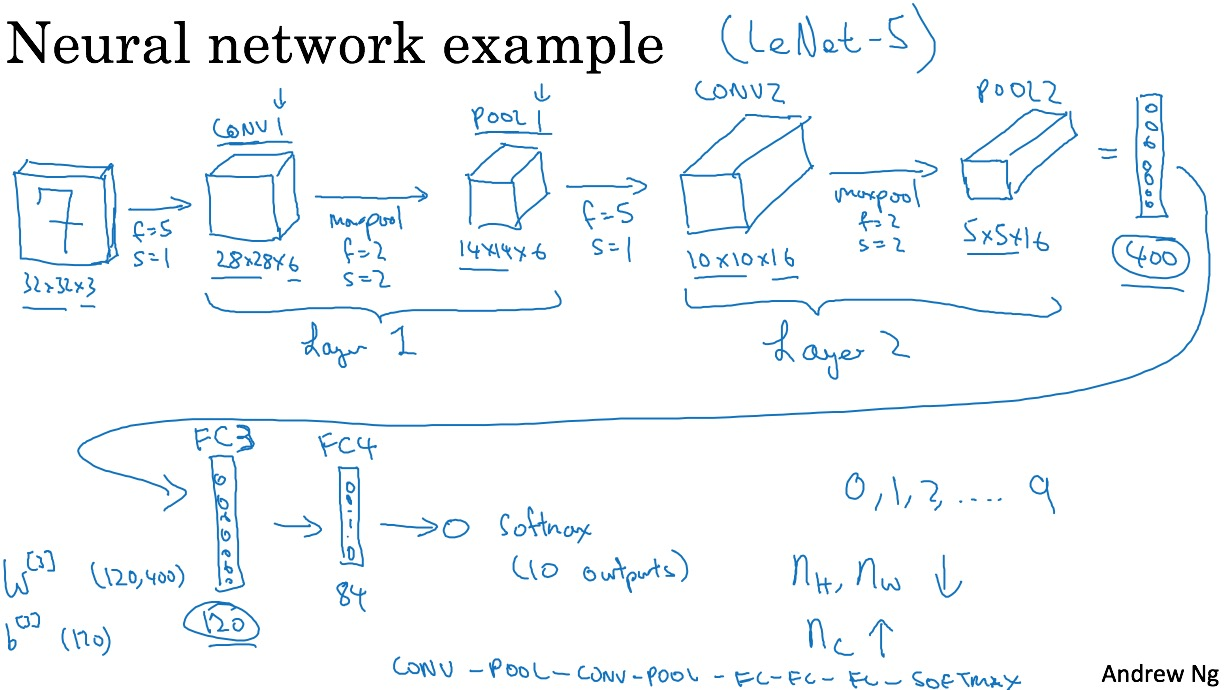
\includegraphics[width=40em]{figures/cnn-example}
    \caption{A CNN example, inspired by LeNet-5}
    \label{fig:cnn-example}
\end{figure}

\begin{figure}[htb]
    \centering
    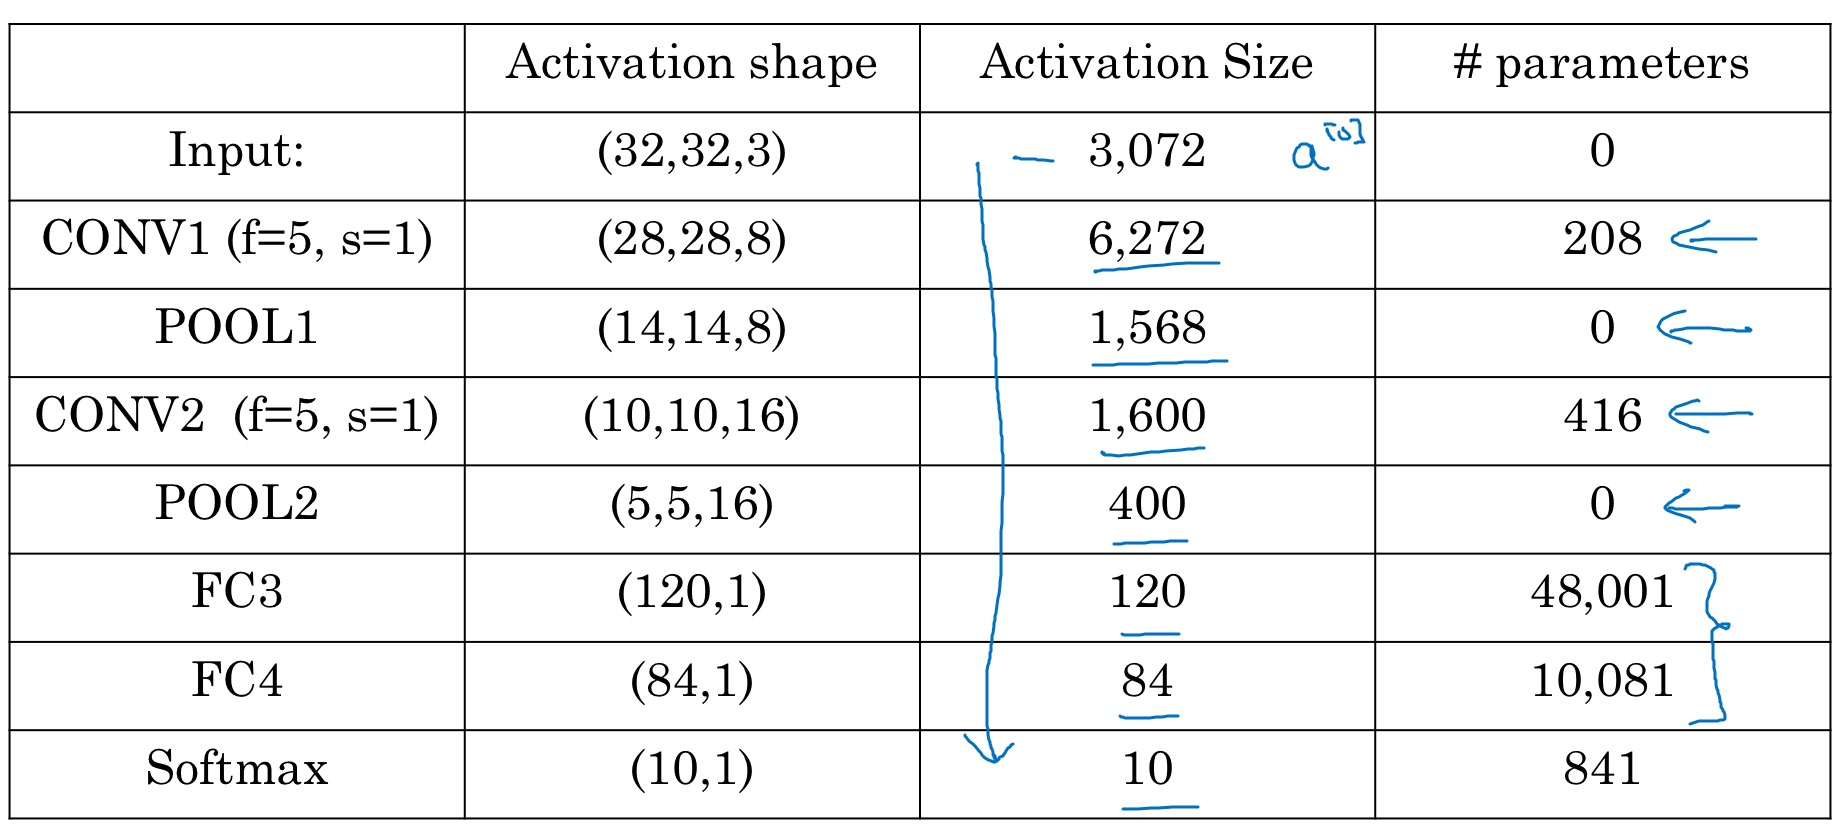
\includegraphics[width=40em]{figures/cnn-example-details}
    \caption{The details of a CNN example, inspired by LeNet-5}
    \label{fig:cnn-example-details}
\end{figure}

\subsubsection{Why Convolutions?}
There are two advantages of convolutional layers over just using fully-connected layers:
\begin{enumerate}
    \item Parameter sharing: A feature detector (such as a vertical edge detector) that's useful in
    one part of the image is probably useful in another part of the image.
    \item Sparsity of connections: In each layer, each output value depends only on a small number
    of inputs.
\end{enumerate}

Convolutional neural networks are very good at capturing translation of the areas, that's because
a convolutional structure helps the neural network encode the fact that an image shifted a few
pixels should result in pretty similar features and should probably be assigned the same output
label.















\end{document}
